\documentclass[a4paper,11pt]{article}
\usepackage{amsmath,amsthm,amsfonts,amssymb,amscd,amstext,vmargin,graphics,graphicx,tabularx,multicol} 
\usepackage[francais]{babel}
\usepackage[utf8]{inputenc}  
\usepackage[T1]{fontenc} 
\usepackage{pstricks-add,tikz,tkz-tab,variations}
\usepackage[autolanguage,np]{numprint} 
\usepackage{color}
\usepackage{ulem}

\setmarginsrb{1.5cm}{0.5cm}{1cm}{0.5cm}{0cm}{0cm}{0cm}{0cm} %Gauche, haut, droite, haut
\newcounter{numexo}
\newcommand{\exo}[1]{\stepcounter{numexo}\noindent{\bf Exercice~\thenumexo} : \marginpar{\hfill /#1}}
\reversemarginpar


\newcounter{enumtabi}
\newcounter{enumtaba}
\newcommand{\q}{\stepcounter{enumtabi} \theenumtabi.  }
\newcommand{\qa}{\stepcounter{enumtaba} (\alph{enumtaba}) }
\newcommand{\initq}{\setcounter{enumtabi}{0}}
\newcommand{\initqa}{\setcounter{enumtaba}{0}}

\newcommand{\be}{\begin{enumerate}}
\newcommand{\ee}{\end{enumerate}}
\newcommand{\bi}{\begin{itemize}}
\newcommand{\ei}{\end{itemize}}
\newcommand{\bp}{\begin{pspicture*}}
\newcommand{\ep}{\end{pspicture*}}
\newcommand{\bt}{\begin{tabular}}
\newcommand{\et}{\end{tabular}}
\renewcommand{\tabularxcolumn}[1]{>{\centering}m{#1}} %(colonne m{} centrée, au lieu de p par défault) 
\newcommand{\tnl}{\tabularnewline}

\newcommand{\bmul}[1]{\begin{multicols}{#1}}
\newcommand{\emul}{\end{multicols}}
\newcommand{\rd}[1]{\textcolor{red}{#1}}

\newcommand{\trait}{\noindent \rule{\linewidth}{0.2mm}}
\newcommand{\hs}[1]{\hspace{#1}}
\newcommand{\vs}[1]{\vspace{#1}}

\newcommand{\N}{\mathbb{N}}
\newcommand{\Z}{\mathbb{Z}}
\newcommand{\R}{\mathbb{R}}
\newcommand{\C}{\mathbb{C}}
\newcommand{\Dcal}{\mathcal{D}}
\newcommand{\Ccal}{\mathcal{C}}
\newcommand{\mc}{\mathcal}

\newcommand{\vect}[1]{\overrightarrow{#1}}
\newcommand{\ds}{\displaystyle}
\newcommand{\eq}{\quad \Leftrightarrow \quad}
\newcommand{\vecti}{\vec{\imath}}
\newcommand{\vectj}{\vec{\jmath}}
\newcommand{\Oij}{(O;\vec{\imath}, \vec{\jmath})}
\newcommand{\OIJ}{(O;I,J)}


\newcommand{\reponse}[1][1]{%
\multido{}{#1}{\makebox[\linewidth]{\rule[0pt]{0pt}{20pt}\dotfill}
}}

\newcommand{\titre}[5] 
% #1: titre #2: haut gauche #3: bas gauche #4: haut droite #5: bas droite
{
\noindent #2 \hfill #4 \\
#3 \hfill #5

\vspace{-1.6cm}

\begin{center}\rule{6cm}{0.5mm}\end{center}
\vspace{0.2cm}
\begin{center}{\large{\textbf{#1}}}\end{center}
\begin{center}\rule{6cm}{0.5mm}\end{center}
}



\begin{document}
\pagestyle{empty}
\titre{Correction du contrôle 1}{3 ème}{}{}{}


\exo{3} Calculer les expressions suivantes et donner la réponse sous la forme d'une fraction irréductible :\\

\bmul{2}

\textcolor{red}{$P = \dfrac{3}{5} \times \dfrac{10}{7} - \dfrac{23}{7} \div \dfrac{1}{7}$ }\\

\textcolor{red}{$P = \dfrac{3\times 2 \times \xout{5}}{7 \times \xout{5}} - \dfrac{23}{7} \times \dfrac{7}{1}$} \\

\textcolor{red}{$P = \dfrac{6}{7 } - \dfrac{161}{7} $ }\\

\fbox {\textcolor{red}{$P = - \dfrac{155}{7} $}} \\

\columnbreak

 \textcolor{red}{$ T = \dfrac{\dfrac{1}{4} + 3}{\dfrac{11}{5}-\dfrac{13}{5}}$  }\\
 
  \textcolor{red}{$ T = \dfrac{\dfrac{1}{4} + \dfrac{3 \times 4}{1 \times 4}}{\dfrac{11-13}{5}}$ } \\
  
   \textcolor{red}{ $ T = \dfrac{\dfrac{1}{4} + \dfrac{12}{4}}{\dfrac{-2}{5}}$ } \\
    
  \textcolor{red}{   $ T =  \dfrac{\dfrac{13}{4}}{\dfrac{-2}{5}}$}  \\
     
    \textcolor{red}{ $ T =  \dfrac{13}{4} \times \dfrac{5}{-2}$ } \\
     
   \fbox{   \textcolor{red}{$ T = - \dfrac{65}{8}$ } }\\

\emul

\exo{6}

On considère la figure ci-dessous sur laquelle (ED)$\slash \slash$(BC) et AB = 7,5 ; BC = 9 ; AC = 6 : AD = 4 ; AG = 10 et AF = 8.


\includegraphics[scale=1]{thales1.eps} \\



\q Calculer AE et ED.\\

\textcolor{red}{Dans les triangles ADE et ACB : on sait que les droites (ED) et (BC) sont parallèles ; que les droites (DC) et (EB) sont sécantes en A et que les points D, A et C sont alignés dans le même ordre que E, A et B.}\\

\textcolor{red}{Selon le théorème de Thalès, on a : \hspace*{0.4cm}$\dfrac{AD}{AC} = \dfrac{AE}{AB} = \dfrac{DE}{BC}$ }\\

\textcolor{red}{On remplace par les données : \hspace*{0.4cm} $\dfrac{4}{6} = \dfrac{AE}{7,5} = \dfrac{DE}{9}$}\\

\textcolor{red}{\underline{- Calcul de AE :}}\\

\textcolor{red}{$\dfrac{4}{6} = \dfrac{AE}{7,5} $ et d'après le produit en croix on a : $AE = \dfrac{4 \times 7,5}{6} = 5 $}\\

\textcolor{red}{Donc \fbox{ AE = 5}}\\

\textcolor{red}{\underline{- Calcul de ED :}}\\

\textcolor{red}{$\dfrac{4}{6} = \dfrac{DE}{9} $ et d'après le produit en croix on a : $DE = \dfrac{4 \times 9}{6} = 6 $}\\

\textcolor{red}{Donc \fbox{ DE = 6 }}\\

\q Prouver que (BC)$\slash \slash$(GF).\\

\textcolor{red}{Dans les triangles ABC et AGF on a : AB = 7,5 ; BC = 9 ; AC = 6 : AD = 4 ; AG = 10 et AF = 8.}\\

\textcolor{red}{ D'une part, $\dfrac{AC}{AF} = \dfrac{6}{8}$ = 0,75}\\

\textcolor{red}{ D'autre part, $\dfrac{AB}{AG} = \dfrac{7,5}{10}$ = 0,75}\\

\textcolor{red}{ $\dfrac{AC}{AF} = \dfrac{AB}{AG}$ et les points A, C et F sont alignés dans le même ordre que A, B et G, d'après la réciproque du théorème de Thalès on peut donc affirmer que les droites (BC) et (GF) sont parallèles. } \\

\exo{3}

\noindent Dans les marais salants, le sel récolté est stocké sur une surface plane.\\
On admet qu'un tas de sel a toujours la forme d'un cône de révolution.\\
Pascal souhaite déterminer la hauteur d'un cône de sel de diamètre 5 mètres. Il possède un bâton de longueur 1 mètre. Il effectue des mesures et réalise les deux schémas ci-dessous.\\


\includegraphics[scale=1]{thales2.eps} 


\initq \q Démontrer que la hauteur de ce cône de sel est égale à 2,5 mètres.\\

\rd{On sait que $ (BC) \perp (AO)$ et que $(SO) \perp (AO)$. Or, deux droites perpendiculaires à une même droite sont parallèles entre elles. Donc $ (BC) \slash \slash (SO)$.}\\

\rd{De plus, les points A, C et S sont alignés dans le même ordre que A,B et O.}\\

\rd{Selon le théorème de Thalès, on a : \hspace*{0.4cm} $\dfrac{AB}{AO} = \dfrac{AC}{AS} = \dfrac{BC}{SO}$}\\

\rd{On remplace par les valeurs connues : $\dfrac{3,20}{8} = \dfrac{AC}{AS} = \dfrac{1}{SO}$}\\

\rd{\underline{On cherche la longueur SO : }}\\

\rd{$\dfrac{3,20}{8} =\dfrac{1}{SO}$ et d'après le produit en croix on a $SO = \dfrac{1 \times 8}{3,20} = 2,5 m$}\\

\rd{Donc \fbox{SO = 2,5 m}}\\


\exo{2,5}

\initq \q Donner tous les diviseurs des nombres entiers suivants : 99; 122.\\

\rd{$D_{99} = \{1; 3 ; 9 ; 11 ; 33 ; 99 \}$ et $D_{122} = \{1; 2 ; 61 ; 122\}$}\\

\q Parmi les six nombres suivants, quels sont ceux qui sont premiers? (\textbf{Justifier votre réponse}.)\\

\rd{Les nombres premiers sont 41, 61 et 71, en effet ce sont les seuls qui ne possèdent que 2 diviseurs.}


\newpage

\exo{3}

Soit $A= 140 $, $ B = 2 \times 3 \times 11$ et $C= 11 \times 13$\\

\initq \q Décomposer A en produit de facteurs premiers.\\

\red $A = 140 = 14 \times 10 = 7 \times 2 \times 2 \times 5$\\
Donc la décomposition en produit de facteurs premiers est $A = 2^{2} \times 5 \times 7$\\

\black \q La fraction $\dfrac{A}{B}$ est-elle irréductible ? (\textbf{Justifier votre réponse}.)\\

\red $\dfrac{A}{B} = \dfrac{2^{2} \times 5 \times 7}{2 \times 3 \times 11}$ donc A et B ont 2 comme facteur commun, on pourra donc simplifier la fraction par 2. La fraction n'est donc pas irréductible.\\

\black \q Même question pour $\dfrac{A}{C}$.(\textbf{Justifier votre réponse}.)\\

\red $\dfrac{A}{C} = \dfrac{2^{2} \times 5 \times 7}{11 \times 13}$ donc A et C n'ont aucun facteur en commun ainsi la fraction est irréductible.\\

\black \exo{2,5} Un confiseur dispose de 966 bonbons aux fruits et 690 caramels. Il souhaite faire des petits paquets tous identiques, en utilisant tous les bonbons et caramels.\\

\initq \q Le confiseur peut-il faire 115 paquets?(\textbf{Justifier votre réponse}.)\\

\red $966 \div 115 = \textbf{8,4}$ et $690 \div 115 = \textbf{6}$ On ne pourra pas faire 115 paquets en utilisant tous les bonbons aux fruits car 115 n'est pas un diviseur de 966. \\

\black \q Quel est le nombre maximal de paquets que le confiseur peut-il réaliser ? Quelle est alors la composition de chaque paquet ?(\textbf{Justifier votre réponse à l'aide d'un calcul de PGCD}.)\\


\red $966 = 3 \times 322 = 3 \times 2 \times 161 = 3 \times 2 \times 7 \times 23$ et $690 = 69 \times 10 = 3 \times 23 \times 2 \times 5  $ Donc $966 = 2 \times 3 \times \textbf{7} \times 23$ et $690 = 2 \times 3 \times \textbf{5} \times 23$.\\

$PGCD(966 ; 690) = 2 \times 3 \times 23 = 138$. Ainsi, on pourra réaliser 138 paquets en utilisant tous les bonbons et caramels. Un paquet contiendra 7 bonbons aux fruits et 5 caramels. (nombres en gras dans la décomposition en produit de facteurs premiers.)\\


\black \exo{Bonus}

On considère la figure ci-dessous sur laquelle:\\
AN vaut le plus grand des facteurs premiers de 33\\
$AC = \dfrac{2 ^ {3} \times 5 \times 11}{8}  $\\
AM vaut le plus grand des diviseurs de 30\\
$ AB = \dfrac{9}{3} \times \dfrac{\dfrac{1}{4} + \dfrac{12}{16}}{\dfrac{0}{3}+\dfrac{1}{10}}$  \\

MN est le PGCD de 36 et de 28

%AN = 11
%AC = 55
%MN = 6
%BC = 30
%AM = 

\includegraphics[scale=1]{thales3_cas_simple.eps} 

\initq \q Démontrer que les droites (MN) et (BC) sont parallèles\\

\q Calculer BC .\\


\end{document}
